\documentclass{article}
\usepackage[utf8]{inputenc}
\usepackage [danish]{babel}
\usepackage[a4paper, hmargin={2.8cm, 2.8cm}, vmargin={2.5cm, 2.5cm}]{geometry}
\usepackage{eso-pic} % \AddToShipoutPicture
\usepackage{graphicx} % \includegraphics
\usepackage [T1]{fontenc}
\usepackage {amsmath}
\usepackage{amsfonts}
\usepackage{amssymb}
\usepackage{setspace}
\usepackage{titlesec}
\usepackage{pgfkeys}
\titleformat{\section}[block]{\Large\bfseries\filcenter}{}{1em}{}
\titleformat{\subsection}[hang]{\bfseries\filcenter}{}{1em}{}
\setcounter{secnumdepth}{0}
\usepackage{pgfgantt}
\setcounter{tocdepth}{3}
\usepackage{graphicx}
\usepackage{geometry}
\usepackage{gensymb}
\usepackage[numbers]{natbib}
\usetikzlibrary{positioning,shapes, shadows, arrows}
\usepackage{tikz}
\usepackage{url}
\linespread{1.2}
\usepackage{fancyhdr}
\pagestyle{fancyplain}
\fancyhead[L]{Bachelor}
\fancyhead[C]{Synopsis}
\fancyhead[R]{23. februar 2015}
\newcommand{\myfl}{\left\lfloor}
\newcommand{\myfr}{\right\rfloor}
\newcommand{\mycl}{\left\lceil}
\newcommand{\mycr}{\right\rceil}

\author{
  \Large{Adam Honoré}
    \\ \texttt{030991-2721}
    \\ \texttt{qgf142@alumni.ku.dk}
  \\ \Large{Alexander Olsen}
    \\ \texttt{200692-2875}
    \\ \texttt{bdj816@alumni.ku.dk}
  \\ \Large{Rasmus Andersen}
    \\ \texttt{200491-2457}
    \\ \texttt{hmd200@alumni.ku.dk} \\
}

\title{
  \vspace{3cm}
  \Huge{Fitts' lov} \\
  \Large{Synopsis}
}
\usepackage{natbib}
\usepackage{graphicx}

\begin{document}

%% Change `ku-farve` to `nat-farve` to use SCIENCE's old colors or
%% `natbio-farve` to use SCIENCE's new colors and logo.
\AddToShipoutPicture*{\put(0,0){\includegraphics*[viewport=0 0 700 600]{natbio-farve}}}
\AddToShipoutPicture*{\put(0,602){\includegraphics*[viewport=0 600 700 1600]{natbio-farve}}}

%% Change `ku-en` to `nat-en` to use the `Faculty of Science` header
\AddToShipoutPicture*{\put(0,0){\includegraphics*{nat-en}}}

\clearpage\maketitle
\thispagestyle{empty}

\newpage

\section{Problemformulering}
Projektet omhandler en empirisk undersøgelse af bevægelsesbaner for pegebevægelser i brugergrænseflader. Der ønskes 

(i) en kort gennemgang af en eller flere udledninger af Fitts' lov; 

(ii) en kort redegørelse for alternative formuleringer af Fitts' lov; 

(iii) en empirisk undersøgelse af et antal brugeres pegebevægelser, herunder logning af bevægelsesbaner, specifikt hastighedsprofiler under hele bevægelsen [denne del vil indebære såvel udvikling af programmel som eksperimenter med brugere]; 

(iv) en statistisk undersøgelse af (a) pegebevægelsernes overensstemmelse med forskellige formuleringer af Fitts' lov og (b) bevægelsesbanernes overenstemmelse med samme.


\section{Begrundelse}
Fitts' lov samt varianter heraf fokuserer kun på længden i mellem målet, målets størrelse og den tid det tager at kommer dertil. Der er inden for HCI-feltet udgivet mange artikler om emnet, men ingen af dem tager højde for pegeredskabets bane for at nå målet, mens kun få artikler kigger på dets acceleration. 

Ingen af de allerede kendte formler for Fitts' lov kan beskrive tiden med 100\% præcision, derfor er der et behov for at undersøge om dette kan optimeres. Vi vil derfor forsøge denne optimering ved at kigge på netop den undervejsliggende bane og acceleration.

\section{Arbejdsopgaver m. tidsplan}
I forbindelse med udarbejdelsen af vores projekt har vi delt det op i etaper, som hver indeholder én hovede arbejdsopgave. En samlet plan kan ses af figur 1.

\subsection{Teoretisk analyse}
Teoretisk gennemgang af Fitts egen lov samt McKenzies, Meyers og Welfords varianter. Et færdigt produkt afspejler sig i et rapport afsnit der indeholder denne gennemgang. Produktet vil blive udarbejdet på baggrund af forfatternes egne artikler samt eventuelle andre relevante. Det forventes at tage cirka 4 uger og skal gerne være færdig d. 5. marts.

\subsection{Design af programmel}
Et gennemovervejet design, som kan bruges ved udarbejdelsen af det programmel vi skal bruge til at teste i. Dette design vil basere sig på ideer fra artikler, som er gennemlæst under den teoretiske analyse. Det er også her blandt andet udviklingsplatform og pegeredskab skal endeligt vælges. Forventes at være færdig på cirka 2 uger med deadline d. 12. marts

\subsection{Programmering}
Udarbejdelsen af et program som vi kan bruge til at indsamle data til at analysere Fitts' lov. Et færdigt produkt er et endeligt program, som kan indsamle data om testdeltagerens baner, hastighed og tid. Forventes at tage cirka 2 uger.

\subsection{Test}
Vores program skal testes af diverse testpersoner, for at indsamle brugbar data. Vi skal som minimum teste 10 deltagere. Det forventes at tage cirka 3 uger.

\subsection{Analyse}
En gennemarbejdet analyse som skal forsøge at beskrive vores indsamlede data ved de forskellige varianter af Fitts' lov, samt forsøge at indarbejde bevægelsesbaner som parameter. Det forventes at tage 3 uger.

\subsection{Finpudsning}
Den endelige rapport skal finpudses, dette inkludere rettelse af stavefejl, sørge for, at rapportafsnittene er sammenhængene osv. Det forventes at tage 1 uge.

\begin{figure}[h]
\centering
\label{fig:tidsplan}
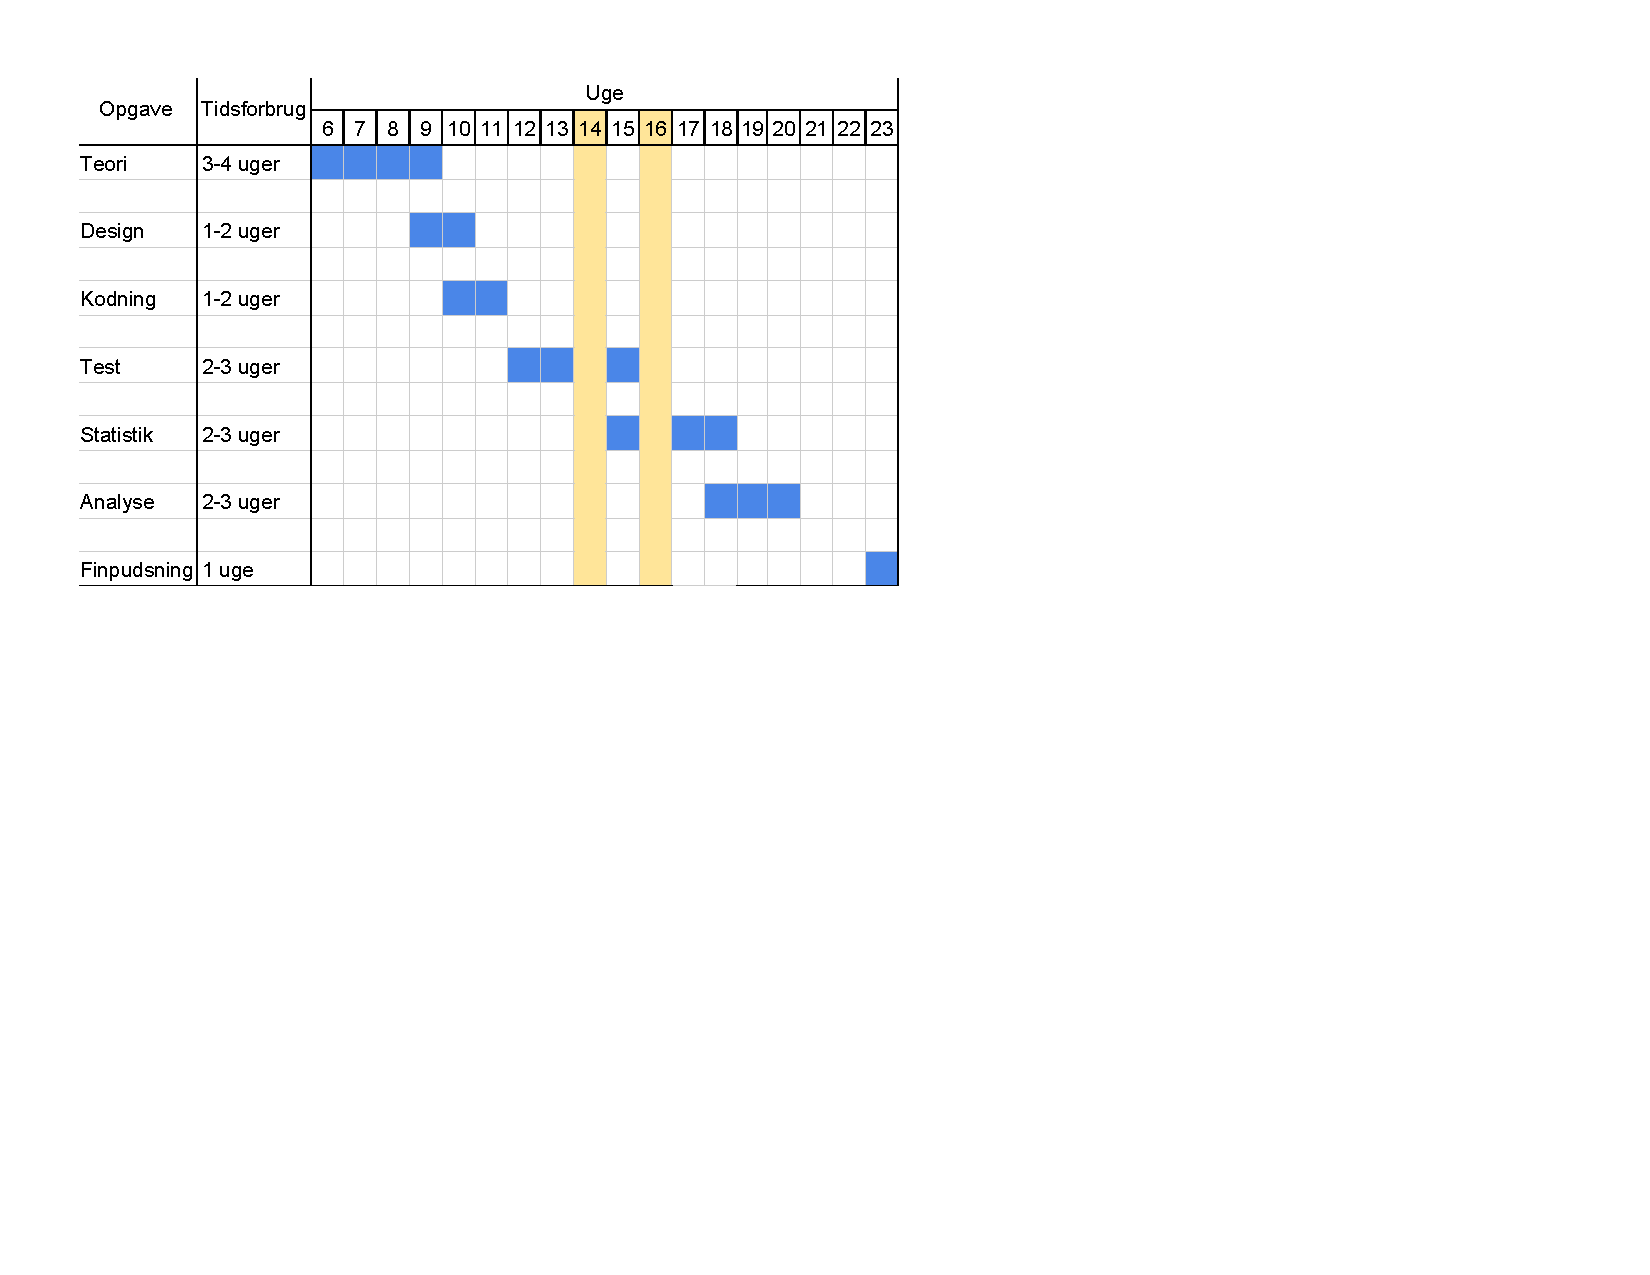
\includegraphics[]{tidsplan.pdf}
\caption{tidsplan}
\end{figure}

\nocite{*}
\newpage
\bibliographystyle{plainnat}
\bibliography{bibliography}

\end{document}